\documentclass[twoside]{book}

% Packages required by doxygen
\usepackage{fixltx2e}
\usepackage{calc}
\usepackage{doxygen}
\usepackage[export]{adjustbox} % also loads graphicx
\usepackage{graphicx}
\usepackage[utf8]{inputenc}
\usepackage{makeidx}
\usepackage{multicol}
\usepackage{multirow}
\PassOptionsToPackage{warn}{textcomp}
\usepackage{textcomp}
\usepackage[nointegrals]{wasysym}
\usepackage[table]{xcolor}

% Font selection
\usepackage[T1]{fontenc}
\usepackage[scaled=.90]{helvet}
\usepackage{courier}
\usepackage{amssymb}
\usepackage{sectsty}
\renewcommand{\familydefault}{\sfdefault}
\allsectionsfont{%
  \fontseries{bc}\selectfont%
  \color{darkgray}%
}
\renewcommand{\DoxyLabelFont}{%
  \fontseries{bc}\selectfont%
  \color{darkgray}%
}
\newcommand{\+}{\discretionary{\mbox{\scriptsize$\hookleftarrow$}}{}{}}

% Page & text layout
\usepackage{geometry}
\geometry{%
  a4paper,%
  top=2.5cm,%
  bottom=2.5cm,%
  left=2.5cm,%
  right=2.5cm%
}
\tolerance=750
\hfuzz=15pt
\hbadness=750
\setlength{\emergencystretch}{15pt}
\setlength{\parindent}{0cm}
\setlength{\parskip}{3ex plus 2ex minus 2ex}
\makeatletter
\renewcommand{\paragraph}{%
  \@startsection{paragraph}{4}{0ex}{-1.0ex}{1.0ex}{%
    \normalfont\normalsize\bfseries\SS@parafont%
  }%
}
\renewcommand{\subparagraph}{%
  \@startsection{subparagraph}{5}{0ex}{-1.0ex}{1.0ex}{%
    \normalfont\normalsize\bfseries\SS@subparafont%
  }%
}
\makeatother

% Headers & footers
\usepackage{fancyhdr}
\pagestyle{fancyplain}
\fancyhead[LE]{\fancyplain{}{\bfseries\thepage}}
\fancyhead[CE]{\fancyplain{}{}}
\fancyhead[RE]{\fancyplain{}{\bfseries\leftmark}}
\fancyhead[LO]{\fancyplain{}{\bfseries\rightmark}}
\fancyhead[CO]{\fancyplain{}{}}
\fancyhead[RO]{\fancyplain{}{\bfseries\thepage}}
\fancyfoot[LE]{\fancyplain{}{}}
\fancyfoot[CE]{\fancyplain{}{}}
\fancyfoot[RE]{\fancyplain{}{\bfseries\scriptsize Generated by Doxygen }}
\fancyfoot[LO]{\fancyplain{}{\bfseries\scriptsize Generated by Doxygen }}
\fancyfoot[CO]{\fancyplain{}{}}
\fancyfoot[RO]{\fancyplain{}{}}
\renewcommand{\footrulewidth}{0.4pt}
\renewcommand{\chaptermark}[1]{%
  \markboth{#1}{}%
}
\renewcommand{\sectionmark}[1]{%
  \markright{\thesection\ #1}%
}

% Indices & bibliography
\usepackage{natbib}
\usepackage[titles]{tocloft}
\setcounter{tocdepth}{3}
\setcounter{secnumdepth}{5}
\makeindex

% Hyperlinks (required, but should be loaded last)
\usepackage{ifpdf}
\ifpdf
  \usepackage[pdftex,pagebackref=true]{hyperref}
\else
  \usepackage[ps2pdf,pagebackref=true]{hyperref}
\fi
\hypersetup{%
  colorlinks=true,%
  linkcolor=blue,%
  citecolor=blue,%
  unicode%
}

% Custom commands
\newcommand{\clearemptydoublepage}{%
  \newpage{\pagestyle{empty}\cleardoublepage}%
}

\usepackage{caption}
\captionsetup{labelsep=space,justification=centering,font={bf},singlelinecheck=off,skip=4pt,position=top}

%===== C O N T E N T S =====

\begin{document}

% Titlepage & ToC
\hypersetup{pageanchor=false,
             bookmarksnumbered=true,
             pdfencoding=unicode
            }
\pagenumbering{roman}
\begin{titlepage}
\vspace*{7cm}
\begin{center}%
{\Large Algo\+\_\+assignment }\\
\vspace*{1cm}
{\large Generated by Doxygen 1.8.11}\\
\end{center}
\end{titlepage}
\clearemptydoublepage
\tableofcontents
\clearemptydoublepage
\pagenumbering{arabic}
\hypersetup{pageanchor=true}

%--- Begin generated contents ---
\chapter{File Index}
\section{File List}
Here is a list of all files with brief descriptions\+:\begin{DoxyCompactList}
\item\contentsline{section}{/home/dhrumil/assignment\+\_\+c/\+Algo\+\_\+assignment/\hyperlink{min__sum_8c}{min\+\_\+sum.\+c} }{\pageref{min__sum_8c}}{}
\item\contentsline{section}{/home/dhrumil/assignment\+\_\+c/\+Algo\+\_\+assignment/\hyperlink{Sample_8c}{Sample.\+c} }{\pageref{Sample_8c}}{}
\item\contentsline{section}{/home/dhrumil/assignment\+\_\+c/\+Algo\+\_\+assignment/\hyperlink{sort_8h}{sort.\+h} }{\pageref{sort_8h}}{}
\item\contentsline{section}{/home/dhrumil/assignment\+\_\+c/\+Algo\+\_\+assignment/\hyperlink{sorting_8c}{sorting.\+c} }{\pageref{sorting_8c}}{}
\end{DoxyCompactList}

\chapter{File Documentation}
\hypertarget{min__sum_8c}{}\section{/home/dhrumil/assignment\+\_\+c/\+Algo\+\_\+assignment/min\+\_\+sum.c File Reference}
\label{min__sum_8c}\index{/home/dhrumil/assignment\+\_\+c/\+Algo\+\_\+assignment/min\+\_\+sum.\+c@{/home/dhrumil/assignment\+\_\+c/\+Algo\+\_\+assignment/min\+\_\+sum.\+c}}
{\ttfamily \#include \char`\"{}sort.\+h\char`\"{}}\\*
{\ttfamily \#include $<$math.\+h$>$}\\*
Include dependency graph for min\+\_\+sum.\+c\+:\nopagebreak
\begin{figure}[H]
\begin{center}
\leavevmode
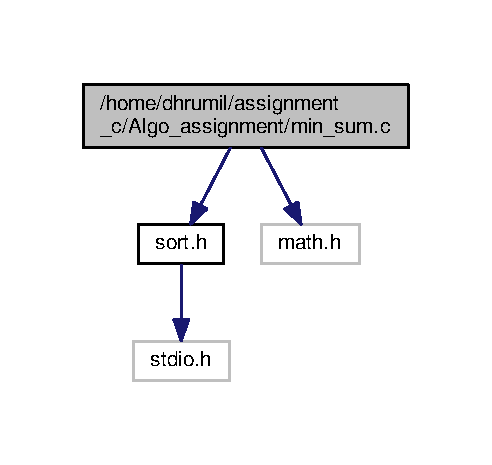
\includegraphics[width=236pt]{min__sum_8c__incl}
\end{center}
\end{figure}
\subsection*{Functions}
\begin{DoxyCompactItemize}
\item 
int \hyperlink{min__sum_8c_ae66f6b31b5ad750f1fe042a706a4e3d4}{main} ()
\begin{DoxyCompactList}\small\item\em Main function of the program. \end{DoxyCompactList}\end{DoxyCompactItemize}


\subsection{Function Documentation}
\index{min\+\_\+sum.\+c@{min\+\_\+sum.\+c}!main@{main}}
\index{main@{main}!min\+\_\+sum.\+c@{min\+\_\+sum.\+c}}
\subsubsection[{\texorpdfstring{main()}{main()}}]{\setlength{\rightskip}{0pt plus 5cm}int main (
\begin{DoxyParamCaption}
{}
\end{DoxyParamCaption}
)}\hypertarget{min__sum_8c_ae66f6b31b5ad750f1fe042a706a4e3d4}{}\label{min__sum_8c_ae66f6b31b5ad750f1fe042a706a4e3d4}


Main function of the program. 

Function main \begin{DoxyDate}{Date}
S\+E\+P/1/2018 
\end{DoxyDate}
\begin{DoxyReturn}{Returns}
int\+: the result of execution. 0\+: success -\/ve\+: on various failures. -\/1\+: if command line is incorrect. 
\end{DoxyReturn}

\hypertarget{Sample_8c}{}\section{/home/dhrumil/assignment\+\_\+c/\+Algo\+\_\+assignment/\+Sample.c File Reference}
\label{Sample_8c}\index{/home/dhrumil/assignment\+\_\+c/\+Algo\+\_\+assignment/\+Sample.\+c@{/home/dhrumil/assignment\+\_\+c/\+Algo\+\_\+assignment/\+Sample.\+c}}
{\ttfamily \#include $<$stdio.\+h$>$}\\*
{\ttfamily \#include $<$stdlib.\+h$>$}\\*
{\ttfamily \#include $<$unistd.\+h$>$}\\*
Include dependency graph for Sample.\+c\+:\nopagebreak
\begin{figure}[H]
\begin{center}
\leavevmode
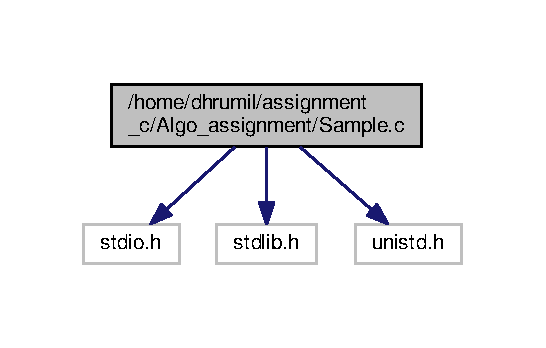
\includegraphics[width=262pt]{Sample_8c__incl}
\end{center}
\end{figure}
\subsection*{Macros}
\begin{DoxyCompactItemize}
\item 
\#define \hyperlink{Sample_8c_af21302abdc020367cb9d4c77eba9bfa7}{D\+E\+F\+\_\+\+O\+U\+T\+\_\+\+L\+EN}~80
\item 
\#define \hyperlink{Sample_8c_a6f67211269e0f3ab8c59a5a94c0fd8ac}{E\+R\+R\+\_\+\+C\+M\+D\+\_\+\+L\+I\+NE}~-\/1
\item 
\#define \hyperlink{Sample_8c_a846551741a0d8ec6d1efd5491798d50d}{E\+R\+R\+\_\+\+F\+I\+LE}~-\/2
\item 
\#define \hyperlink{Sample_8c_adb83721d9bb6486d78a52f27db60eba9}{E\+R\+R\+O\+R\+\_\+\+D\+I\+SP}~printf
\end{DoxyCompactItemize}
\subsection*{Functions}
\begin{DoxyCompactItemize}
\item 
int \hyperlink{Sample_8c_acd99c1f214798d6f71f54fae793e9c00}{parse\+Cmd\+Line} (int argc, char $\ast$argv\mbox{[}$\,$\mbox{]})
\begin{DoxyCompactList}\small\item\em Parses the commnad line options. \end{DoxyCompactList}\item 
int \hyperlink{Sample_8c_a6ca3699b06fef35baf0349d8641f8288}{fold\+Line} (char $\ast$in\+Buf, unsigned long bytes\+To\+Read)
\begin{DoxyCompactList}\small\item\em Folds each line exceeding a certain limit into shorter lines. \end{DoxyCompactList}\item 
int \hyperlink{Sample_8c_af8cb7e4491718bc4504f864fcb909324}{process\+Lines} ()
\begin{DoxyCompactList}\small\item\em Main function of the program. \end{DoxyCompactList}\item 
void \hyperlink{Sample_8c_aead97c99e70c0da7036fbbe230ef68b6}{print\+Usage} ()
\begin{DoxyCompactList}\small\item\em Prints the usage of this program. \end{DoxyCompactList}\item 
void \hyperlink{Sample_8c_a631d78806ec72c285cd1fff6f5afde13}{release\+Resources} ()
\begin{DoxyCompactList}\small\item\em Closes all open resources. \end{DoxyCompactList}\item 
int \hyperlink{Sample_8c_a0ddf1224851353fc92bfbff6f499fa97}{main} (int argc, char $\ast$argv\mbox{[}$\,$\mbox{]})
\begin{DoxyCompactList}\small\item\em Main function of the program. \end{DoxyCompactList}\end{DoxyCompactItemize}
\subsection*{Variables}
\begin{DoxyCompactItemize}
\item 
unsigned long \hyperlink{Sample_8c_a938c33cabaf53e9be65c0b022680c550}{max\+Out\+Len}
\item 
F\+I\+LE $\ast$ \hyperlink{Sample_8c_aefd8ef723553b9975c9879b191221ef3}{in\+File\+Ptr}
\item 
F\+I\+LE $\ast$ \hyperlink{Sample_8c_a127e7fd3047998f98386afdfb2471989}{out\+File\+Ptr}
\item 
char $\ast$ \hyperlink{Sample_8c_a68895d33cec4d40fa3e38cb4452e0d58}{input\+File\+Name}
\item 
char $\ast$ \hyperlink{Sample_8c_ac224b2769f256d5f706fde4c2fc17a11}{output\+File\+Name}
\end{DoxyCompactItemize}


\subsection{Macro Definition Documentation}
\index{Sample.\+c@{Sample.\+c}!D\+E\+F\+\_\+\+O\+U\+T\+\_\+\+L\+EN@{D\+E\+F\+\_\+\+O\+U\+T\+\_\+\+L\+EN}}
\index{D\+E\+F\+\_\+\+O\+U\+T\+\_\+\+L\+EN@{D\+E\+F\+\_\+\+O\+U\+T\+\_\+\+L\+EN}!Sample.\+c@{Sample.\+c}}
\subsubsection[{\texorpdfstring{D\+E\+F\+\_\+\+O\+U\+T\+\_\+\+L\+EN}{DEF_OUT_LEN}}]{\setlength{\rightskip}{0pt plus 5cm}\#define D\+E\+F\+\_\+\+O\+U\+T\+\_\+\+L\+EN~80}\hypertarget{Sample_8c_af21302abdc020367cb9d4c77eba9bfa7}{}\label{Sample_8c_af21302abdc020367cb9d4c77eba9bfa7}
\index{Sample.\+c@{Sample.\+c}!E\+R\+R\+\_\+\+C\+M\+D\+\_\+\+L\+I\+NE@{E\+R\+R\+\_\+\+C\+M\+D\+\_\+\+L\+I\+NE}}
\index{E\+R\+R\+\_\+\+C\+M\+D\+\_\+\+L\+I\+NE@{E\+R\+R\+\_\+\+C\+M\+D\+\_\+\+L\+I\+NE}!Sample.\+c@{Sample.\+c}}
\subsubsection[{\texorpdfstring{E\+R\+R\+\_\+\+C\+M\+D\+\_\+\+L\+I\+NE}{ERR_CMD_LINE}}]{\setlength{\rightskip}{0pt plus 5cm}\#define E\+R\+R\+\_\+\+C\+M\+D\+\_\+\+L\+I\+NE~-\/1}\hypertarget{Sample_8c_a6f67211269e0f3ab8c59a5a94c0fd8ac}{}\label{Sample_8c_a6f67211269e0f3ab8c59a5a94c0fd8ac}
\index{Sample.\+c@{Sample.\+c}!E\+R\+R\+\_\+\+F\+I\+LE@{E\+R\+R\+\_\+\+F\+I\+LE}}
\index{E\+R\+R\+\_\+\+F\+I\+LE@{E\+R\+R\+\_\+\+F\+I\+LE}!Sample.\+c@{Sample.\+c}}
\subsubsection[{\texorpdfstring{E\+R\+R\+\_\+\+F\+I\+LE}{ERR_FILE}}]{\setlength{\rightskip}{0pt plus 5cm}\#define E\+R\+R\+\_\+\+F\+I\+LE~-\/2}\hypertarget{Sample_8c_a846551741a0d8ec6d1efd5491798d50d}{}\label{Sample_8c_a846551741a0d8ec6d1efd5491798d50d}
\index{Sample.\+c@{Sample.\+c}!E\+R\+R\+O\+R\+\_\+\+D\+I\+SP@{E\+R\+R\+O\+R\+\_\+\+D\+I\+SP}}
\index{E\+R\+R\+O\+R\+\_\+\+D\+I\+SP@{E\+R\+R\+O\+R\+\_\+\+D\+I\+SP}!Sample.\+c@{Sample.\+c}}
\subsubsection[{\texorpdfstring{E\+R\+R\+O\+R\+\_\+\+D\+I\+SP}{ERROR_DISP}}]{\setlength{\rightskip}{0pt plus 5cm}\#define E\+R\+R\+O\+R\+\_\+\+D\+I\+SP~printf}\hypertarget{Sample_8c_adb83721d9bb6486d78a52f27db60eba9}{}\label{Sample_8c_adb83721d9bb6486d78a52f27db60eba9}


\subsection{Function Documentation}
\index{Sample.\+c@{Sample.\+c}!fold\+Line@{fold\+Line}}
\index{fold\+Line@{fold\+Line}!Sample.\+c@{Sample.\+c}}
\subsubsection[{\texorpdfstring{fold\+Line(char $\ast$in\+Buf, unsigned long bytes\+To\+Read)}{foldLine(char *inBuf, unsigned long bytesToRead)}}]{\setlength{\rightskip}{0pt plus 5cm}int fold\+Line (
\begin{DoxyParamCaption}
\item[{char $\ast$}]{in\+Buf, }
\item[{unsigned long}]{bytes\+To\+Read}
\end{DoxyParamCaption}
)}\hypertarget{Sample_8c_a6ca3699b06fef35baf0349d8641f8288}{}\label{Sample_8c_a6ca3699b06fef35baf0349d8641f8288}


Folds each line exceeding a certain limit into shorter lines. 

Function fold\+Line \begin{DoxyDate}{Date}
J\+U\+L/16/2018 
\end{DoxyDate}

\begin{DoxyParams}{Parameters}
{\em char} & $\ast$\+: buffer to process unsigned long\+: Bytes to read \\
\hline
\end{DoxyParams}
\begin{DoxyReturn}{Returns}
int\+: the remaining characters to output from current line. 
\end{DoxyReturn}
\index{Sample.\+c@{Sample.\+c}!main@{main}}
\index{main@{main}!Sample.\+c@{Sample.\+c}}
\subsubsection[{\texorpdfstring{main(int argc, char $\ast$argv[])}{main(int argc, char *argv[])}}]{\setlength{\rightskip}{0pt plus 5cm}int main (
\begin{DoxyParamCaption}
\item[{int}]{argc, }
\item[{char $\ast$}]{argv\mbox{[}$\,$\mbox{]}}
\end{DoxyParamCaption}
)}\hypertarget{Sample_8c_a0ddf1224851353fc92bfbff6f499fa97}{}\label{Sample_8c_a0ddf1224851353fc92bfbff6f499fa97}


Main function of the program. 

Function main \begin{DoxyDate}{Date}
J\+U\+L/16/2018 
\end{DoxyDate}

\begin{DoxyParams}{Parameters}
{\em int} & argc\+: \# of command line arguments char $\ast$\+: argv\+: the char array to hold each command line arg. \\
\hline
\end{DoxyParams}
\begin{DoxyReturn}{Returns}
int\+: the result of execution. 0\+: success -\/ve\+: on various failures. -\/1\+: if command line is incorrect. 
\end{DoxyReturn}
\index{Sample.\+c@{Sample.\+c}!parse\+Cmd\+Line@{parse\+Cmd\+Line}}
\index{parse\+Cmd\+Line@{parse\+Cmd\+Line}!Sample.\+c@{Sample.\+c}}
\subsubsection[{\texorpdfstring{parse\+Cmd\+Line(int argc, char $\ast$argv[])}{parseCmdLine(int argc, char *argv[])}}]{\setlength{\rightskip}{0pt plus 5cm}int parse\+Cmd\+Line (
\begin{DoxyParamCaption}
\item[{int}]{argc, }
\item[{char $\ast$}]{argv\mbox{[}$\,$\mbox{]}}
\end{DoxyParamCaption}
)}\hypertarget{Sample_8c_acd99c1f214798d6f71f54fae793e9c00}{}\label{Sample_8c_acd99c1f214798d6f71f54fae793e9c00}


Parses the commnad line options. 

Function parse\+Cmd\+Line \begin{DoxyDate}{Date}
D\+E\+C/11/2008 
\end{DoxyDate}

\begin{DoxyParams}{Parameters}
{\em int} & argc\+: \# of command line arguments char $\ast$\+: argv\+: the char array to hold each command line arg. \\
\hline
\end{DoxyParams}
\begin{DoxyReturn}{Returns}
int\+: the result of execution. 0\+: success -\/ve\+: on various failures. 
\end{DoxyReturn}
\index{Sample.\+c@{Sample.\+c}!print\+Usage@{print\+Usage}}
\index{print\+Usage@{print\+Usage}!Sample.\+c@{Sample.\+c}}
\subsubsection[{\texorpdfstring{print\+Usage()}{printUsage()}}]{\setlength{\rightskip}{0pt plus 5cm}void print\+Usage (
\begin{DoxyParamCaption}
{}
\end{DoxyParamCaption}
)}\hypertarget{Sample_8c_aead97c99e70c0da7036fbbe230ef68b6}{}\label{Sample_8c_aead97c99e70c0da7036fbbe230ef68b6}


Prints the usage of this program. 

Function print\+Usage \begin{DoxyDate}{Date}
J\+U\+L/16/2018 
\end{DoxyDate}

\begin{DoxyParams}{Parameters}
{\em None} & \\
\hline
\end{DoxyParams}
\begin{DoxyReturn}{Returns}
None 
\end{DoxyReturn}
\index{Sample.\+c@{Sample.\+c}!process\+Lines@{process\+Lines}}
\index{process\+Lines@{process\+Lines}!Sample.\+c@{Sample.\+c}}
\subsubsection[{\texorpdfstring{process\+Lines()}{processLines()}}]{\setlength{\rightskip}{0pt plus 5cm}int process\+Lines (
\begin{DoxyParamCaption}
{}
\end{DoxyParamCaption}
)}\hypertarget{Sample_8c_af8cb7e4491718bc4504f864fcb909324}{}\label{Sample_8c_af8cb7e4491718bc4504f864fcb909324}


Main function of the program. 

Function process\+Lines \begin{DoxyDate}{Date}
J\+U\+L/16/2018 
\end{DoxyDate}

\begin{DoxyParams}{Parameters}
{\em None} & \\
\hline
\end{DoxyParams}
\begin{DoxyReturn}{Returns}
int\+: the result of execution. 0\+: success -\/ve\+: on various failures. 
\end{DoxyReturn}
\index{Sample.\+c@{Sample.\+c}!release\+Resources@{release\+Resources}}
\index{release\+Resources@{release\+Resources}!Sample.\+c@{Sample.\+c}}
\subsubsection[{\texorpdfstring{release\+Resources()}{releaseResources()}}]{\setlength{\rightskip}{0pt plus 5cm}void release\+Resources (
\begin{DoxyParamCaption}
{}
\end{DoxyParamCaption}
)}\hypertarget{Sample_8c_a631d78806ec72c285cd1fff6f5afde13}{}\label{Sample_8c_a631d78806ec72c285cd1fff6f5afde13}


Closes all open resources. 

Function release\+Resources \begin{DoxyDate}{Date}
J\+U\+L/16/2018 
\end{DoxyDate}

\begin{DoxyParams}{Parameters}
{\em None} & \\
\hline
\end{DoxyParams}
\begin{DoxyReturn}{Returns}
None 
\end{DoxyReturn}


\subsection{Variable Documentation}
\index{Sample.\+c@{Sample.\+c}!in\+File\+Ptr@{in\+File\+Ptr}}
\index{in\+File\+Ptr@{in\+File\+Ptr}!Sample.\+c@{Sample.\+c}}
\subsubsection[{\texorpdfstring{in\+File\+Ptr}{inFilePtr}}]{\setlength{\rightskip}{0pt plus 5cm}F\+I\+LE$\ast$ in\+File\+Ptr}\hypertarget{Sample_8c_aefd8ef723553b9975c9879b191221ef3}{}\label{Sample_8c_aefd8ef723553b9975c9879b191221ef3}
\index{Sample.\+c@{Sample.\+c}!input\+File\+Name@{input\+File\+Name}}
\index{input\+File\+Name@{input\+File\+Name}!Sample.\+c@{Sample.\+c}}
\subsubsection[{\texorpdfstring{input\+File\+Name}{inputFileName}}]{\setlength{\rightskip}{0pt plus 5cm}char$\ast$ input\+File\+Name}\hypertarget{Sample_8c_a68895d33cec4d40fa3e38cb4452e0d58}{}\label{Sample_8c_a68895d33cec4d40fa3e38cb4452e0d58}
\index{Sample.\+c@{Sample.\+c}!max\+Out\+Len@{max\+Out\+Len}}
\index{max\+Out\+Len@{max\+Out\+Len}!Sample.\+c@{Sample.\+c}}
\subsubsection[{\texorpdfstring{max\+Out\+Len}{maxOutLen}}]{\setlength{\rightskip}{0pt plus 5cm}unsigned long max\+Out\+Len}\hypertarget{Sample_8c_a938c33cabaf53e9be65c0b022680c550}{}\label{Sample_8c_a938c33cabaf53e9be65c0b022680c550}
\index{Sample.\+c@{Sample.\+c}!out\+File\+Ptr@{out\+File\+Ptr}}
\index{out\+File\+Ptr@{out\+File\+Ptr}!Sample.\+c@{Sample.\+c}}
\subsubsection[{\texorpdfstring{out\+File\+Ptr}{outFilePtr}}]{\setlength{\rightskip}{0pt plus 5cm}F\+I\+LE$\ast$ out\+File\+Ptr}\hypertarget{Sample_8c_a127e7fd3047998f98386afdfb2471989}{}\label{Sample_8c_a127e7fd3047998f98386afdfb2471989}
\index{Sample.\+c@{Sample.\+c}!output\+File\+Name@{output\+File\+Name}}
\index{output\+File\+Name@{output\+File\+Name}!Sample.\+c@{Sample.\+c}}
\subsubsection[{\texorpdfstring{output\+File\+Name}{outputFileName}}]{\setlength{\rightskip}{0pt plus 5cm}char$\ast$ output\+File\+Name}\hypertarget{Sample_8c_ac224b2769f256d5f706fde4c2fc17a11}{}\label{Sample_8c_ac224b2769f256d5f706fde4c2fc17a11}

\hypertarget{sort_8h}{}\section{/home/dhrumil/assignment\+\_\+c/\+Algo\+\_\+assignment/sort.h File Reference}
\label{sort_8h}\index{/home/dhrumil/assignment\+\_\+c/\+Algo\+\_\+assignment/sort.\+h@{/home/dhrumil/assignment\+\_\+c/\+Algo\+\_\+assignment/sort.\+h}}
{\ttfamily \#include $<$stdio.\+h$>$}\\*
Include dependency graph for sort.\+h\+:\nopagebreak
\begin{figure}[H]
\begin{center}
\leavevmode
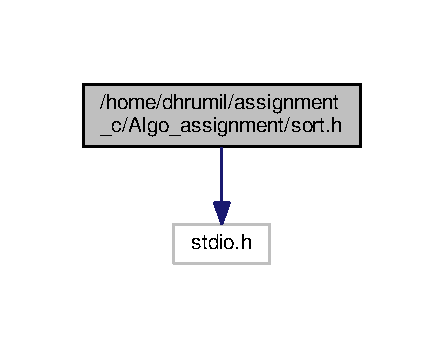
\includegraphics[width=213pt]{sort_8h__incl}
\end{center}
\end{figure}
This graph shows which files directly or indirectly include this file\+:\nopagebreak
\begin{figure}[H]
\begin{center}
\leavevmode
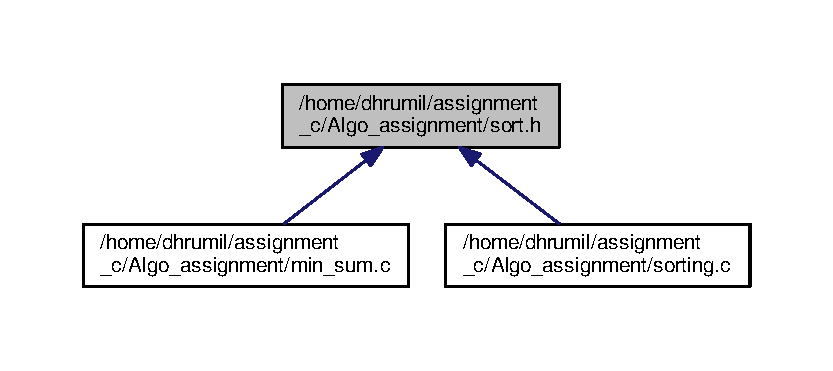
\includegraphics[width=350pt]{sort_8h__dep__incl}
\end{center}
\end{figure}
\subsection*{Functions}
\begin{DoxyCompactItemize}
\item 
void \hyperlink{sort_8h_ade02f829b69e6f3dc0728a94d506c12f}{fill\+Array\+Default} (int arr\mbox{[}$\,$\mbox{]}, int n)
\begin{DoxyCompactList}\small\item\em To fill the array with zero. \end{DoxyCompactList}\item 
void \hyperlink{sort_8h_abaf0d87927ec93821fc0638a996df362}{fill\+Array} (int arr\mbox{[}$\,$\mbox{]}, int n)
\begin{DoxyCompactList}\small\item\em To fill the array with user input. \end{DoxyCompactList}\item 
void \hyperlink{sort_8h_a0dfb41e81ff64e73d8af6a76c96a2e63}{swap} (int $\ast$n1, int $\ast$n2)
\begin{DoxyCompactList}\small\item\em To swap two number. \end{DoxyCompactList}\item 
void \hyperlink{sort_8h_ae8bb50a1a6f0f873bf2c91dd4adf4a1a}{selection\+Sort} (int arr\mbox{[}$\,$\mbox{]}, int n)
\begin{DoxyCompactList}\small\item\em To sort data using selection sort. \end{DoxyCompactList}\item 
void \hyperlink{sort_8h_a80a64c660726e8cfc7f933482004210f}{bubble\+Sort} (int arr\mbox{[}$\,$\mbox{]}, int n)
\begin{DoxyCompactList}\small\item\em To sort data using bubble sort algorithm. \end{DoxyCompactList}\item 
void \hyperlink{sort_8h_a3fde3e15492d674dbd6caf7c061a2b35}{insertion\+Sort} (int arr\mbox{[}$\,$\mbox{]}, int n)
\begin{DoxyCompactList}\small\item\em To sort data using insertion sort algoritm. \end{DoxyCompactList}\item 
int \hyperlink{sort_8h_a9309b42f2d8f51655338b408c3cee05b}{find\+Max} (int arr\mbox{[}$\,$\mbox{]}, int n)
\begin{DoxyCompactList}\small\item\em To find maximux number from data. \end{DoxyCompactList}\item 
void \hyperlink{sort_8h_a764c5d8b08ed437b88d8ab9148777b67}{count\+Sort} (int arr\mbox{[}$\,$\mbox{]}, int n, int digit)
\begin{DoxyCompactList}\small\item\em To sort data using perticular digit in number. \end{DoxyCompactList}\item 
void \hyperlink{sort_8h_a60a1e52389125e77c9b652383d863369}{rad\+Sort} (int arr\mbox{[}$\,$\mbox{]}, int n)
\begin{DoxyCompactList}\small\item\em To sort data using radix sort algorithm. \end{DoxyCompactList}\item 
void \hyperlink{sort_8h_aeb95eb63a0e297446db588c6c236a7f0}{radix\+Sort} (int arr\mbox{[}$\,$\mbox{]}, int n)
\begin{DoxyCompactList}\small\item\em To sort nagative and positive number sepereatally using radix sort. \end{DoxyCompactList}\item 
int \hyperlink{sort_8h_a2f0658d814c1e14b49d419add95c79b9}{partition} (int arr\mbox{[}$\,$\mbox{]}, int low, int high)
\begin{DoxyCompactList}\small\item\em To partition array and return postion where it is partitioned. \end{DoxyCompactList}\item 
void \hyperlink{sort_8h_a6deda3bd254bf5da0c533d0a02b81922}{quick\+Sort} (int arr\mbox{[}$\,$\mbox{]}, int low, int high)
\begin{DoxyCompactList}\small\item\em To sort the data using quick sort algorithm. \end{DoxyCompactList}\item 
void \hyperlink{sort_8h_ac2a8c8437419a08047fafbe4e9f1a3dd}{print\+Array} (int arr\mbox{[}$\,$\mbox{]}, int size)
\begin{DoxyCompactList}\small\item\em To print array. \end{DoxyCompactList}\end{DoxyCompactItemize}


\subsection{Function Documentation}
\index{sort.\+h@{sort.\+h}!bubble\+Sort@{bubble\+Sort}}
\index{bubble\+Sort@{bubble\+Sort}!sort.\+h@{sort.\+h}}
\subsubsection[{\texorpdfstring{bubble\+Sort(int arr[], int n)}{bubbleSort(int arr[], int n)}}]{\setlength{\rightskip}{0pt plus 5cm}void bubble\+Sort (
\begin{DoxyParamCaption}
\item[{int}]{arr\mbox{[}$\,$\mbox{]}, }
\item[{int}]{n}
\end{DoxyParamCaption}
)}\hypertarget{sort_8h_a80a64c660726e8cfc7f933482004210f}{}\label{sort_8h_a80a64c660726e8cfc7f933482004210f}


To sort data using bubble sort algorithm. 

Function bubble\+Sort \begin{DoxyDate}{Date}
A\+U\+G/31/2018 
\end{DoxyDate}

\begin{DoxyParams}{Parameters}
{\em int} & arr\mbox{[}\mbox{]}\+: stored data int\+: n\+: size of data. \\
\hline
\end{DoxyParams}
\begin{DoxyReturn}{Returns}
void 
\end{DoxyReturn}
\index{sort.\+h@{sort.\+h}!count\+Sort@{count\+Sort}}
\index{count\+Sort@{count\+Sort}!sort.\+h@{sort.\+h}}
\subsubsection[{\texorpdfstring{count\+Sort(int arr[], int n, int digit)}{countSort(int arr[], int n, int digit)}}]{\setlength{\rightskip}{0pt plus 5cm}void count\+Sort (
\begin{DoxyParamCaption}
\item[{int}]{arr\mbox{[}$\,$\mbox{]}, }
\item[{int}]{n, }
\item[{int}]{digit}
\end{DoxyParamCaption}
)}\hypertarget{sort_8h_a764c5d8b08ed437b88d8ab9148777b67}{}\label{sort_8h_a764c5d8b08ed437b88d8ab9148777b67}


To sort data using perticular digit in number. 

Function count\+Sort \begin{DoxyDate}{Date}
A\+U\+G/31/2018 
\end{DoxyDate}

\begin{DoxyParams}{Parameters}
{\em int} & arr\mbox{[}\mbox{]}\+: stored data int\+: n\+: size of data. \\
\hline
\end{DoxyParams}
\begin{DoxyReturn}{Returns}
void 
\end{DoxyReturn}
\index{sort.\+h@{sort.\+h}!fill\+Array@{fill\+Array}}
\index{fill\+Array@{fill\+Array}!sort.\+h@{sort.\+h}}
\subsubsection[{\texorpdfstring{fill\+Array(int arr[], int n)}{fillArray(int arr[], int n)}}]{\setlength{\rightskip}{0pt plus 5cm}void fill\+Array (
\begin{DoxyParamCaption}
\item[{int}]{arr\mbox{[}$\,$\mbox{]}, }
\item[{int}]{n}
\end{DoxyParamCaption}
)}\hypertarget{sort_8h_abaf0d87927ec93821fc0638a996df362}{}\label{sort_8h_abaf0d87927ec93821fc0638a996df362}


To fill the array with user input. 

Function fill\+Array \begin{DoxyDate}{Date}
A\+U\+G/31/2018 
\end{DoxyDate}

\begin{DoxyParams}{Parameters}
{\em int} & arr\mbox{[}\mbox{]}\+: stored data int\+: n\+: size of data. \\
\hline
\end{DoxyParams}
\begin{DoxyReturn}{Returns}
void 
\end{DoxyReturn}
\index{sort.\+h@{sort.\+h}!fill\+Array\+Default@{fill\+Array\+Default}}
\index{fill\+Array\+Default@{fill\+Array\+Default}!sort.\+h@{sort.\+h}}
\subsubsection[{\texorpdfstring{fill\+Array\+Default(int arr[], int n)}{fillArrayDefault(int arr[], int n)}}]{\setlength{\rightskip}{0pt plus 5cm}void fill\+Array\+Default (
\begin{DoxyParamCaption}
\item[{int}]{arr\mbox{[}$\,$\mbox{]}, }
\item[{int}]{n}
\end{DoxyParamCaption}
)}\hypertarget{sort_8h_ade02f829b69e6f3dc0728a94d506c12f}{}\label{sort_8h_ade02f829b69e6f3dc0728a94d506c12f}


To fill the array with zero. 

Function fill\+Array\+Default \begin{DoxyDate}{Date}
A\+U\+G/31/2018 
\end{DoxyDate}

\begin{DoxyParams}{Parameters}
{\em int} & arr\mbox{[}\mbox{]}\+: stored data int\+: n\+: size of data. \\
\hline
\end{DoxyParams}
\begin{DoxyReturn}{Returns}
void 
\end{DoxyReturn}
\index{sort.\+h@{sort.\+h}!find\+Max@{find\+Max}}
\index{find\+Max@{find\+Max}!sort.\+h@{sort.\+h}}
\subsubsection[{\texorpdfstring{find\+Max(int arr[], int n)}{findMax(int arr[], int n)}}]{\setlength{\rightskip}{0pt plus 5cm}int find\+Max (
\begin{DoxyParamCaption}
\item[{int}]{arr\mbox{[}$\,$\mbox{]}, }
\item[{int}]{n}
\end{DoxyParamCaption}
)}\hypertarget{sort_8h_a9309b42f2d8f51655338b408c3cee05b}{}\label{sort_8h_a9309b42f2d8f51655338b408c3cee05b}


To find maximux number from data. 

Function find\+Max \begin{DoxyDate}{Date}
A\+U\+G/31/2018 
\end{DoxyDate}

\begin{DoxyParams}{Parameters}
{\em int} & arr\mbox{[}\mbox{]}\+: stored data int\+: n\+: size of data. \\
\hline
\end{DoxyParams}
\begin{DoxyReturn}{Returns}
void 
\end{DoxyReturn}
\index{sort.\+h@{sort.\+h}!insertion\+Sort@{insertion\+Sort}}
\index{insertion\+Sort@{insertion\+Sort}!sort.\+h@{sort.\+h}}
\subsubsection[{\texorpdfstring{insertion\+Sort(int arr[], int n)}{insertionSort(int arr[], int n)}}]{\setlength{\rightskip}{0pt plus 5cm}void insertion\+Sort (
\begin{DoxyParamCaption}
\item[{int}]{arr\mbox{[}$\,$\mbox{]}, }
\item[{int}]{n}
\end{DoxyParamCaption}
)}\hypertarget{sort_8h_a3fde3e15492d674dbd6caf7c061a2b35}{}\label{sort_8h_a3fde3e15492d674dbd6caf7c061a2b35}


To sort data using insertion sort algoritm. 

Function insertion\+Sort \begin{DoxyDate}{Date}
A\+U\+G/31/2018 
\end{DoxyDate}

\begin{DoxyParams}{Parameters}
{\em int} & arr\mbox{[}\mbox{]}\+: stored data int\+: n\+: size of data. \\
\hline
\end{DoxyParams}
\begin{DoxyReturn}{Returns}
void 
\end{DoxyReturn}
\index{sort.\+h@{sort.\+h}!partition@{partition}}
\index{partition@{partition}!sort.\+h@{sort.\+h}}
\subsubsection[{\texorpdfstring{partition(int arr[], int low, int high)}{partition(int arr[], int low, int high)}}]{\setlength{\rightskip}{0pt plus 5cm}int partition (
\begin{DoxyParamCaption}
\item[{int}]{arr\mbox{[}$\,$\mbox{]}, }
\item[{int}]{low, }
\item[{int}]{high}
\end{DoxyParamCaption}
)}\hypertarget{sort_8h_a2f0658d814c1e14b49d419add95c79b9}{}\label{sort_8h_a2f0658d814c1e14b49d419add95c79b9}


To partition array and return postion where it is partitioned. 

Function partition \begin{DoxyDate}{Date}
A\+U\+G/31/2018 
\end{DoxyDate}

\begin{DoxyParams}{Parameters}
{\em int} & arr\mbox{[}\mbox{]}\+: stored data int\+: n\+: size of data. \\
\hline
\end{DoxyParams}
\begin{DoxyReturn}{Returns}
int \+: postion where it is partitioned. 
\end{DoxyReturn}
\index{sort.\+h@{sort.\+h}!print\+Array@{print\+Array}}
\index{print\+Array@{print\+Array}!sort.\+h@{sort.\+h}}
\subsubsection[{\texorpdfstring{print\+Array(int arr[], int size)}{printArray(int arr[], int size)}}]{\setlength{\rightskip}{0pt plus 5cm}void print\+Array (
\begin{DoxyParamCaption}
\item[{int}]{arr\mbox{[}$\,$\mbox{]}, }
\item[{int}]{size}
\end{DoxyParamCaption}
)}\hypertarget{sort_8h_ac2a8c8437419a08047fafbe4e9f1a3dd}{}\label{sort_8h_ac2a8c8437419a08047fafbe4e9f1a3dd}


To print array. 

print\+Array \begin{DoxyDate}{Date}
A\+U\+G/31/2018 
\end{DoxyDate}

\begin{DoxyParams}{Parameters}
{\em int} & arr\mbox{[}\mbox{]}\+: stored data int\+: n\+: size of data. \\
\hline
\end{DoxyParams}
\begin{DoxyReturn}{Returns}
void 
\end{DoxyReturn}
\index{sort.\+h@{sort.\+h}!quick\+Sort@{quick\+Sort}}
\index{quick\+Sort@{quick\+Sort}!sort.\+h@{sort.\+h}}
\subsubsection[{\texorpdfstring{quick\+Sort(int arr[], int low, int high)}{quickSort(int arr[], int low, int high)}}]{\setlength{\rightskip}{0pt plus 5cm}void quick\+Sort (
\begin{DoxyParamCaption}
\item[{int}]{arr\mbox{[}$\,$\mbox{]}, }
\item[{int}]{low, }
\item[{int}]{high}
\end{DoxyParamCaption}
)}\hypertarget{sort_8h_a6deda3bd254bf5da0c533d0a02b81922}{}\label{sort_8h_a6deda3bd254bf5da0c533d0a02b81922}


To sort the data using quick sort algorithm. 

quick\+Sort \begin{DoxyDate}{Date}
A\+U\+G/31/2018 
\end{DoxyDate}

\begin{DoxyParams}{Parameters}
{\em int} & arr\mbox{[}\mbox{]}\+: stored data int\+: n\+: size of data. \\
\hline
\end{DoxyParams}
\begin{DoxyReturn}{Returns}
void 
\end{DoxyReturn}
\index{sort.\+h@{sort.\+h}!radix\+Sort@{radix\+Sort}}
\index{radix\+Sort@{radix\+Sort}!sort.\+h@{sort.\+h}}
\subsubsection[{\texorpdfstring{radix\+Sort(int arr[], int n)}{radixSort(int arr[], int n)}}]{\setlength{\rightskip}{0pt plus 5cm}void radix\+Sort (
\begin{DoxyParamCaption}
\item[{int}]{arr\mbox{[}$\,$\mbox{]}, }
\item[{int}]{n}
\end{DoxyParamCaption}
)}\hypertarget{sort_8h_aeb95eb63a0e297446db588c6c236a7f0}{}\label{sort_8h_aeb95eb63a0e297446db588c6c236a7f0}


To sort nagative and positive number sepereatally using radix sort. 

Function radix\+Sort \begin{DoxyDate}{Date}
A\+U\+G/31/2018 
\end{DoxyDate}

\begin{DoxyParams}{Parameters}
{\em int} & arr\mbox{[}\mbox{]}\+: stored data int\+: n\+: size of data. \\
\hline
\end{DoxyParams}
\begin{DoxyReturn}{Returns}
void 
\end{DoxyReturn}
\index{sort.\+h@{sort.\+h}!rad\+Sort@{rad\+Sort}}
\index{rad\+Sort@{rad\+Sort}!sort.\+h@{sort.\+h}}
\subsubsection[{\texorpdfstring{rad\+Sort(int arr[], int n)}{radSort(int arr[], int n)}}]{\setlength{\rightskip}{0pt plus 5cm}void rad\+Sort (
\begin{DoxyParamCaption}
\item[{int}]{arr\mbox{[}$\,$\mbox{]}, }
\item[{int}]{n}
\end{DoxyParamCaption}
)}\hypertarget{sort_8h_a60a1e52389125e77c9b652383d863369}{}\label{sort_8h_a60a1e52389125e77c9b652383d863369}


To sort data using radix sort algorithm. 

Function red\+Sort \begin{DoxyDate}{Date}
A\+U\+G/31/2018 
\end{DoxyDate}

\begin{DoxyParams}{Parameters}
{\em int} & arr\mbox{[}\mbox{]}\+: stored data int\+: n\+: size of data. \\
\hline
\end{DoxyParams}
\begin{DoxyReturn}{Returns}
void 
\end{DoxyReturn}
\index{sort.\+h@{sort.\+h}!selection\+Sort@{selection\+Sort}}
\index{selection\+Sort@{selection\+Sort}!sort.\+h@{sort.\+h}}
\subsubsection[{\texorpdfstring{selection\+Sort(int arr[], int n)}{selectionSort(int arr[], int n)}}]{\setlength{\rightskip}{0pt plus 5cm}void selection\+Sort (
\begin{DoxyParamCaption}
\item[{int}]{arr\mbox{[}$\,$\mbox{]}, }
\item[{int}]{n}
\end{DoxyParamCaption}
)}\hypertarget{sort_8h_ae8bb50a1a6f0f873bf2c91dd4adf4a1a}{}\label{sort_8h_ae8bb50a1a6f0f873bf2c91dd4adf4a1a}


To sort data using selection sort. 

Function selection\+Sort \begin{DoxyDate}{Date}
A\+U\+G/31/2018 
\end{DoxyDate}

\begin{DoxyParams}{Parameters}
{\em int} & arr\mbox{[}\mbox{]}\+: stored data int\+: n\+: size of data. \\
\hline
\end{DoxyParams}
\begin{DoxyReturn}{Returns}
void 
\end{DoxyReturn}
\index{sort.\+h@{sort.\+h}!swap@{swap}}
\index{swap@{swap}!sort.\+h@{sort.\+h}}
\subsubsection[{\texorpdfstring{swap(int $\ast$n1, int $\ast$n2)}{swap(int *n1, int *n2)}}]{\setlength{\rightskip}{0pt plus 5cm}void swap (
\begin{DoxyParamCaption}
\item[{int $\ast$}]{n1, }
\item[{int $\ast$}]{n2}
\end{DoxyParamCaption}
)}\hypertarget{sort_8h_a0dfb41e81ff64e73d8af6a76c96a2e63}{}\label{sort_8h_a0dfb41e81ff64e73d8af6a76c96a2e63}


To swap two number. 

Function swap \begin{DoxyDate}{Date}
A\+U\+G/31/2018 
\end{DoxyDate}

\begin{DoxyParams}{Parameters}
{\em int$\ast$} & \+: n1\+: first number to swap. int$\ast$ \+: n2\+: second number to swap. \\
\hline
\end{DoxyParams}
\begin{DoxyReturn}{Returns}
void. 
\end{DoxyReturn}

\hypertarget{sorting_8c}{}\section{/home/dhrumil/assignment\+\_\+c/\+Algo\+\_\+assignment/sorting.c File Reference}
\label{sorting_8c}\index{/home/dhrumil/assignment\+\_\+c/\+Algo\+\_\+assignment/sorting.\+c@{/home/dhrumil/assignment\+\_\+c/\+Algo\+\_\+assignment/sorting.\+c}}
{\ttfamily \#include \char`\"{}sort.\+h\char`\"{}}\\*
{\ttfamily \#include $<$time.\+h$>$}\\*
{\ttfamily \#include $<$stdlib.\+h$>$}\\*
Include dependency graph for sorting.\+c\+:\nopagebreak
\begin{figure}[H]
\begin{center}
\leavevmode
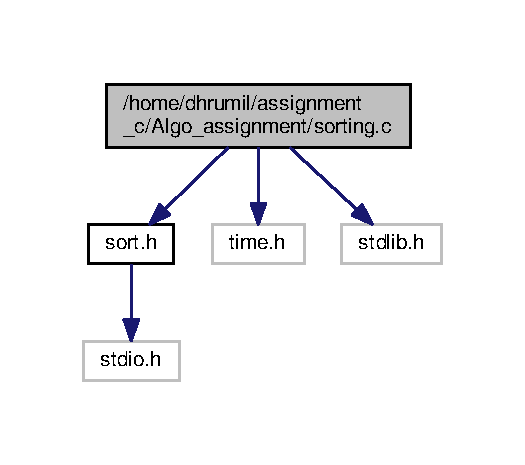
\includegraphics[width=252pt]{sorting_8c__incl}
\end{center}
\end{figure}
\subsection*{Functions}
\begin{DoxyCompactItemize}
\item 
int \hyperlink{sorting_8c_ae66f6b31b5ad750f1fe042a706a4e3d4}{main} ()
\begin{DoxyCompactList}\small\item\em Main function of the program. \end{DoxyCompactList}\end{DoxyCompactItemize}


\subsection{Function Documentation}
\index{sorting.\+c@{sorting.\+c}!main@{main}}
\index{main@{main}!sorting.\+c@{sorting.\+c}}
\subsubsection[{\texorpdfstring{main()}{main()}}]{\setlength{\rightskip}{0pt plus 5cm}int main (
\begin{DoxyParamCaption}
{}
\end{DoxyParamCaption}
)}\hypertarget{sorting_8c_ae66f6b31b5ad750f1fe042a706a4e3d4}{}\label{sorting_8c_ae66f6b31b5ad750f1fe042a706a4e3d4}


Main function of the program. 

Function main \begin{DoxyDate}{Date}
A\+U\+G/91/2018 
\end{DoxyDate}
\begin{DoxyReturn}{Returns}
int\+: the result of execution. 0\+: success -\/ve\+: on various failures. -\/1\+: if command line is incorrect. 
\end{DoxyReturn}
$<$ To store size of data

$<$ To store the data

$<$ to make choice 
%--- End generated contents ---

% Index
\backmatter
\newpage
\phantomsection
\clearemptydoublepage
\addcontentsline{toc}{chapter}{Index}
\printindex

\end{document}
